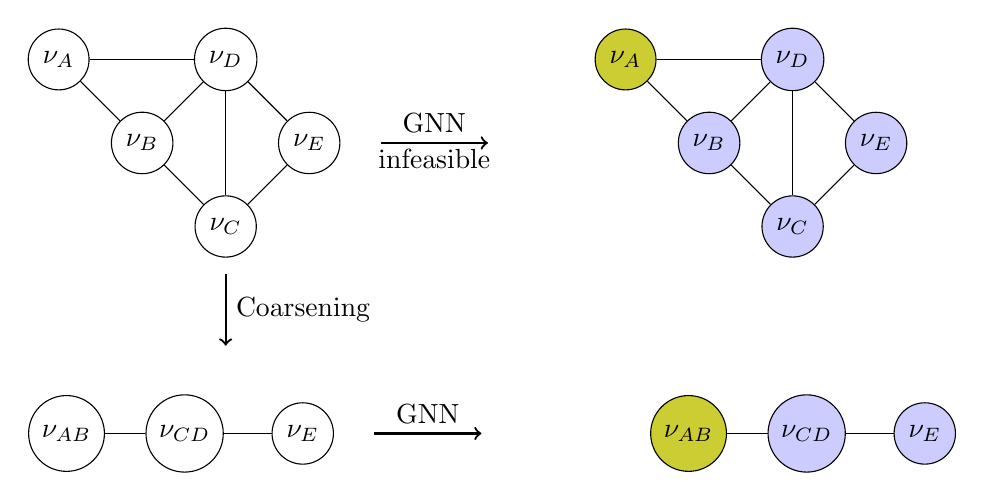
\begin{tikzpicture}
\tikzset{classA/.style={circle, draw=black, fill=blue!20!yellow}, node distance=1.5cm}
\tikzset{classB/.style={circle, draw=black, fill=blue!20}, node distance=1.5cm}
\tikzset{class0/.style={circle, draw=black, fill=white}, node distance=1.5cm}
  \begin{scope}
    \node[class0] (A) {$\nu_{A}$};
    \node[class0, below right of=A] (B) {$\nu_{B}$};
    \node[class0, below right of=B] (C) {$\nu_{C}$};
    \node[class0, above right of=B] (D) {$\nu_{D}$};
    \node[class0, below right of=D] (E) {$\nu_{E}$};
    \draw [-] (A) -- (B) ;
    \draw [-] (A) -- (D) ;
    \draw [-] (C) -- (D) ;
    \draw [-] (D) -- (E) ; 
    \draw [-] (C) -- (E) ;  
    \draw [-] (C) -- (B) ;    
    \draw [-] (D) -- (B) ;
    \draw[->, thick] ([xshift=6ex] E.center) -- ([xshift=15ex] E.center) node [pos=0.5, above] (oGNN) {GNN}; \
    \node[below of=oGNN, node distance=3ex]{\alert{infeasible}};
    \uncover<2->{
        \draw[->, thick] ([yshift=-4ex] C.center) -- ([yshift=-10ex] C.center) node [pos=0.5, right] (ocoars) {Coarsening};
    }
  \end{scope}

  \begin{scope}[xshift=7.2cm, yshift=0cm]
    \node[classA] (A) {$\nu_{A}$};
    \node[classB, below right of=A] (B) {$\nu_{B}$};
    \node[classB, below right of=B] (C) {$\nu_{C}$};
    \node[classB, above right of=B] (D) {$\nu_{D}$};
    \node[classB, below right of=D] (E) {$\nu_{E}$};
    \draw [-] (A) -- (B) ;
    \draw [-] (A) -- (D) ;
    \draw [-] (C) -- (D) ;
    \draw [-] (D) -- (E) ; 
    \draw [-] (C) -- (E) ;  
    \draw [-] (C) -- (B) ;    
    \draw [-] (D) -- (B) ;   
    % \uncover<3->{\node[above of=D, node distance=4ex]{{\color{green} good performance}};}    
  \end{scope} 

\uncover<2->{
    \begin{scope}[yshift=-4.75cm, xshift=0.1cm]
        \node[class0] (AB) {$\nu_{AB}$};
    \node[class0, right of=AB] (CD) {$\nu_{CD}$};
    \node[class0, right of=CD] (E) {$\nu_{E}$};
    \draw [-] (AB) -- (CD);
    \draw [-] (CD) -- (E); 
    \uncover<3->{
        \draw[->, thick] ([xshift=6ex] E.center) -- ([xshift=15ex] E.center) node [pos=0.5, above] (oGNN) {GNN};
    }
    % \uncover<2->{\node[below of=oGNN, node distance=3ex]{{\color{green} simplified}};}
  \end{scope}
  }
  
  \uncover<3->{
    \begin{scope}[yshift=-4.75cm, xshift=8cm]
        \node[classA] (AB) {$\nu_{AB}$};
    \node[classB, right of=AB] (CD) {$\nu_{CD}$};
    \node[classB, right of=CD] (E) {$\nu_{E}$};
    \draw [-] (AB) -- (CD);
    \draw [-] (CD) -- (E);
    % \uncover<3->{\node[below of=CD, node distance=4ex]{{\color{red} worse performance}};}
    \end{scope}
}
 \end{tikzpicture}
